\IEEEraisesectionheading{\section{Introduction}\label{sec:introduction}}
  

Humans are faced with a stream of high-dimensional sensory inputs and minimal external supervision, and yet, are able to learn a range of complex, generalizable skills and behaviors.
While there has been significant progress in developing deep reinforcement learning algorithms that learn complex skills and scale to high-dimensional observation spaces, such as pixels~\cite{tdgammon,atari,e2e,alphago}, learning behaviors that \emph{generalize} to new tasks and objects remains an open problem.
The key to generalization is diversity. When deployed in a narrow, closed-world environment, a reinforcement learning algorithm will recover skills that are successful only in a narrow range of settings. 
Learning skills in diverse  environments, such as the real world, presents a number of significant challenges: external reward feedback is extremely sparse or non-existent, and the agent has only indirect access to the state of the world through its senses, which, in the case of a robot, might correspond to cameras and joint encoders.


We approach the problem of learning generalizable behavior in the real world from the standpoint of sensory prediction. Prediction is often considered a fundamental component of intelligence. Through prediction, it is possible to learn useful concepts about the world even from a raw stream of sensory observations, such as images from a camera. If we predict raw sensory observations directly, we do not need to assume availability of low-dimensional state information or an extrinsic reward signal.  Image observations are both information-rich and high-dimensional, presenting both an opportunity and a challenge. Future observations provide a substantial amount of supervisory information for a machine learning algorithm. However, the predictive model must have the capacity to predict these high-dimensional observations, and the control algorithm must be able to use such a model to effectively select actions to accomplish human-specified goals.  Examples of such goals are shown in figure \ref{fig:example_traj}.


%Instead of focusing on mastery of highly-specialized skills in closed-world environments, here we focus on \emph{generalization} in diverse environments.
%%SL.09.03: this is an important and critical sentence, but I don't like that we from the outset present it in contrast to something so negative (those other guys fail at this, but we don't) -- just say what we do well, and then talk about alternatives. I think we can motivate the work and explain the challenge without necessarily getting so bogged down in the failure of prior work.
We study control via prediction in the context of robotic manipulation, formulating a model-based reinforcement learning approach centered around prediction of raw sensory observations. One of the biggest challenges in learning-based robotic manipulation is generalization: how can we learn models that are useful not just for a narrow range of tasks seen during training, but that can be used to perform new tasks with new objects that were not seen previously?
Collecting a training dataset that is sufficiently rich and diverse is often challenging in highly-structured robotics experiments, which depend on human intervention for reward signals, resets, and safety constraints. We instead set up a minimally structured robotic control domain, where data is collected by the robot via unsupervised interaction with a wide range of objects, making it practical to collect large amounts of interaction data. The robot collects a stream of raw sensory observations (image pixels), without any reward signal at training time, and without the ability to reset the environment between episodes. This setting is both realistic and necessary for studying RL in diverse real-world environments, as it enables automated and unattended collection of diverse interaction experience. Since the training setting affords no readily accessible reward signal, learning by prediction presents an appealing option: the supervision signal for prediction is always available even in the stream of unsupervised experience.
We therefore propose to learn action-conditioned predictive models directly on raw pixel observations, and show that they can be used to accomplish a range of pixel-based manipulation tasks on a real robot in the physical world at test-time. 

%%CF.11.04: Deleted the below since it seemed repetitive
%Sensory prediction models are goal-agnostic, which enables learning for a variety of different goals at the same time. 
%By learning from raw sensor readings, they are also fully general, in that they do not require access to any other state representation beyond the observations. %%CF: This above sentence is repetitive 
%Our overall approach amounts to a deep model-based reinforcement learning algorithm that leverages video prediction models to perform a variety of pixel-based control tasks.
%In addition the practicality of leveraging the only available supervision in such sparse reward environments, sensory prediciton models are also goal-agnostic, which enables learning for a variety of different goals.
%% TODO - motivate why not to learn a model on top of a more abstract representation of the observations? [The supervision, inherently, comes from the same place.]
%TODO - motivate why raw pixels rather than more compact representation (because pixels contain complete information -- can give Sergey's crossing-the-street example -- and pixels are the only thing that is readily available; also pixels contain more supervision)
%Despite the benefits, a number of challenges arise when aiming to use sensory prediction models: how can we learn a model of high-dimensional observations, and how should an objective or reward be determined with respect to the predicted observations? %how should experience be collected? %how should actions be chosen with respect to the model?
%We discuss each of these design decisions and propose several options, weighting the benefits and trade-offs of each.
%Our overall approach amounts to a deep model-based reinforcement learning algorithm that leverages video prediction models to achieve a variety of pixel-based control tasks without shaped reward information.
The main contributions of this work are as follows. We present \emph{visual MPC}, a general framework for deep reinforcement learning with sensory prediction models that is suitable for learning behaviors in diverse, open-world environments (see figure~\ref{fig:overview}).
We describe deep neural network architectures that are effective for predicting pixel-level observations amid occlusions and with novel objects. Unlike low-dimensional representations of state, specifying and evaluating the reward from pixel predictions at test-time is nontrivial: we present several practical methods for specifying and evaluating progress towards the goal---including distances to goal pixel positions, registration to goal images, and image classifiers---and compare their effectiveness and use-cases.
%, abstracting away the model architecture %, the policy optimization,
%and the form of the reward function with respect to predicted observations.
Finally, our evaluation shows how these components can be combined to enable a real robot to perform a range of object manipulation tasks from raw pixel observations. Our experiments include manipulation of previously unseen objects, handling multiple objects, pushing objects around obstructions, handling clutter, manipulating deformable objects such as cloth, recovering from large perturbations, and grasping and maneuvering objects to user-specified locations in 3D-space. Our results represent a significant advance in the \emph{generality} of skills that can be acquired by a real robot operating on raw pixel values using a single model.

This article combines and extends material from several prior conference papers~\cite{foresight,sna,ebert2018robustness,flo}, presenting them in the context of a unified system. We include additional experiments, including cloth manipulation and placing tasks, a quantitative \emph{multi-task} experiment assessing the performance of our method on a wide range of distinct tasks with a single model, as well as a comprehensive, open-sourced simulation environment to facilitate future research and better reproducibility. The code and videos can be found on the following webpage\footnote{For videos \& code: \url{https://sites.google.com/view/visualforesight}}.
%%SL.10.15: make sure we actually have all this :)
%%SL.11.21: Try to avoid using the term "benchmark" to refer to quantitative experiments. The connotation in robotics and ML is that "benchmark" refers to a standardized test used across a range of papers, so it is confusing to call it a benchmark if no one has done a test like this before. You can call it a quantitative experiment or a quantitative comparison.

\begin{figure}[t]
\centering
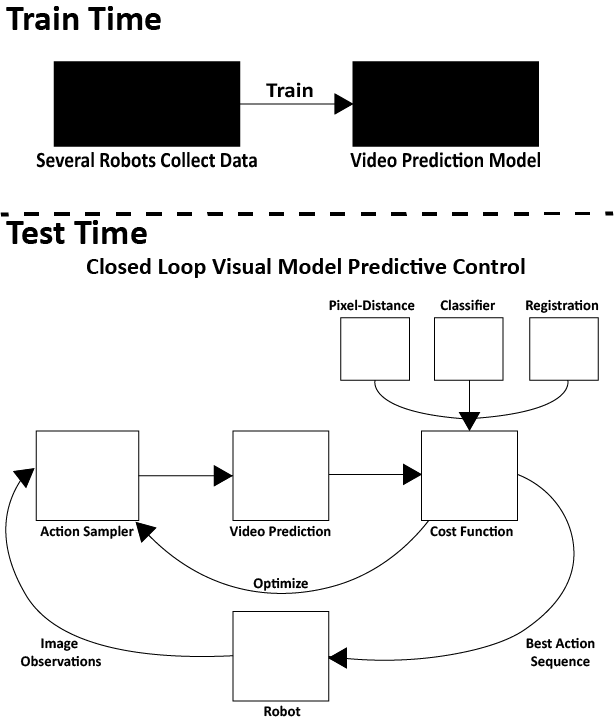
\includegraphics[width=\columnwidth,trim={0mm 0 0 0},clip]{images_general/overview_roughdraft.png}
\caption{\small{Overview of visual MPC. At training time (top) interaction data is collected autonomously and used to train a video-prediction model. At test time (bottom) this model is used for sampling-based planning. In this work we discuss three different choices for the planning objective.}}
\label{fig:overview}
\end{figure}




 





